\section{Introduction}
%Motivation
\begin{frame}
    \frametitle{Introduction -- Motivation}
    \begin{block}{Tunable Antennas}
      \begin{itemize}
      \item Even though smartphones has begun to grow in physical size, less space is allocated for the antennas.
      \item LTE standard requiresterminals to operate in a wide range of frequencies (650-2700)
      \item MIMO is a large part of LTE, which increases the number of antennas on the device 
      \item Able to make smaller antennas that can cover more bands.
      \item Approched in a very pratical manner with theory in mind. 
      \item Simple simulations and then actual prototypes.
      \end{itemize}
    \end{block}
\vspace*{-0.5cm}
  \begin{center} 
   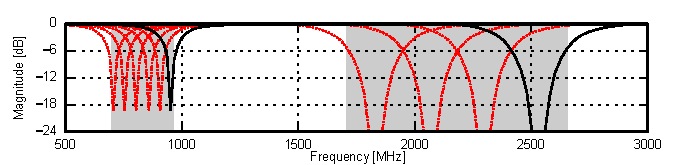
\includegraphics[width=\textwidth]{img/henrik/reconfsweep}
  \end{center}
\end{frame}
%System overview 
\begin{frame}
    \frametitle{Introduction -- A System Perspective}
  \begin{center} 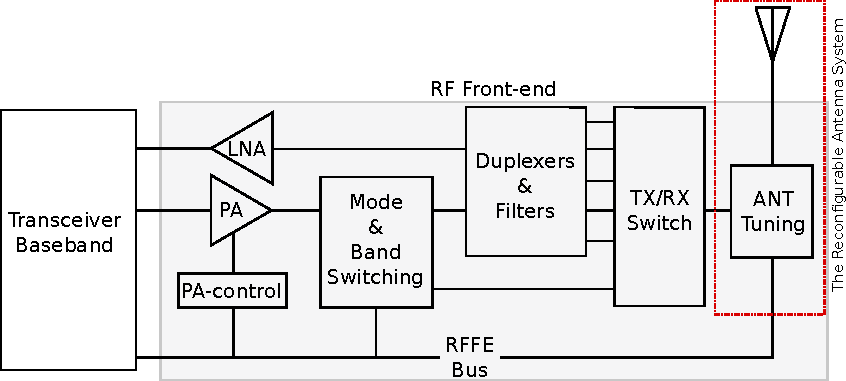
\includegraphics[scale=0.8]{img/henrik/system_diagram}
  \end{center}
\end{frame}


%Problem anal
\section{Problem Analysis}
\begin{frame}[fragile]
    \frametitle{Initial Problem Analysis}
    \vspace*{-0.5cm}
    \begin{columns}[onlytextwidth,t]
        \column{0.49\linewidth}
    \begin{block}{Topics}
          \begin{itemize}
          \item Mobile standards
          \item LTE
          \item Basic Antenna Theory
          \item Matching circuits \& Tuners
          \item Propagations Models
          \end{itemize}
    \end{block}
        \column{0.49\linewidth}
    \begin{block}{}
          \begin{itemize}
          \item User effects
          \item MIMO in Handsets
          \item Maxwell's Equations
          \item FDTD 
          \item Test Equipment and methods
          \end{itemize}
    \end{block}
    \end{columns}
    \begin{block}{Outcome of Analysis}
      \begin{itemize}
      \item Covering all the specified bands is indeed a problem
      \item Can be solved with frequency reconfigurability
      \item Correlation and isolation are important parameters for MIMO-capacity
      \item Many different types of tuners, we chose RF-mems capacitors
      \end{itemize}
    \end{block}
\end{frame}

%System overview 
\begin{frame}
    \frametitle{Requirement specification}

    \begin{block}{Functional Requirements}
    \centering
    {\tiny
\begin{tabularx}{\linewidth}{|l|X|}
    \hline
    ID & Requirement \\
    \hline
    \freq{dualband} & The antenna system must consist of two single-feed dual-band antennas covering the bands described in Requirement~\sreqref{fbands}. \\
    \freq{updownlink} & Each antenna must cover both uplink and downlink at the same time for each required LTE band.\\
    % \freq{usereffect} & Must be able to re-tune any detuning due to user effects. \\ % ???? HAHA
    \freq{matching} & Must have a simple matching network, containing a variable capacitor for tuning inside the specified bands.\\
    \freq{wispry} & Must use a WiSpry WS1040 MEMS variable capacitor chip in the matching network.\\
    \hline
\end{tabularx}

    }
    \end{block}

    \begin{block}{Specific Requirements}
    \centering
    {\tiny
\begin{tabularx}{\linewidth}{|l|l|X|}
    \hline
    ID & Specification & Requirement \\
    \hline
    \sreq{fbands} & Frequency bands\slash tunable range & \num{700}--\SI{960}{MHz}, \num{1710}--\SI{2170}{MHz}, \num{2300}--\SI{2400}{MHz}, \num{2550}--\SI{2650}{MHz} \\
    \sreq{bandwidthlow} & Minimum tunable bandwidth (\num{700}--\SI{960}{MHz}) & \SI{80}{MHz} (band 8) \\
    \sreq{bandwidthhigh} & Minimum tunable bandwidth (\num{1710}--\SI{2650}{MHz}) & \SI{720}{MHz} (band 15) \\
    \sreq{physdim} & Physical dimensions & External: $70\times140\times7$\,\si{mm\cubed}, PCB: $55\times120\times1.6$\,\si{mm\cubed} (FR-4)\\
    \sreq{copper} & Ground plane copper thickness & \SI{0.035}{mm} \\
    \sreq{retloss} & In-band return loss (impedance bandwidth) & $\text{RL} > \SI{6}{dB}$\\
    \sreq{correlation} & In-band correlation between antenna elements (correlation bandwidth) & $\rho_e < 0.5$\\
    \sreq{efficiency} & In-band total efficiency in free-space (efficiency bandwidth)  & $>\SI{50}{\%}$ \\
    \sreq{sar} & Maximum SAR & \SI{2}{W\per kg} averaged over \SI{10}{g} of tissue\\
    \sreq{tunable} & Tunable capacitor range (WS1040)& \SI{0.3}{pF} to \SI{2.9}{pF} in steps of \SI{0.2}{pF} (\SI{0.1}{pF} minimum)  \\
    \sreq{ltepower} & Reference power level  & \SI{23}{dBm} (\SI{0.2}{W})\\
    \hline
\end{tabularx}

    }
    \end{block}

    \begin{block}{Test Specification}    
      \begin{itemize}
      \item For each specific requirement is a given test specification
      \end{itemize}
    \end{block}
\end{frame}

\section{Technical Solution}
\begin{frame}
    \frametitle{Technical Solution -- Introduction}
    \begin{block}{Three different antenna designs}
      \begin{itemize}
      \item Initial designs did not have to fully comply with the requirements
      \item Some based on previous designs from published papers
      \item Simplified simulations
      \end{itemize}
    \end{block}
\vspace*{-0.5cm}
  \begin{center} 
    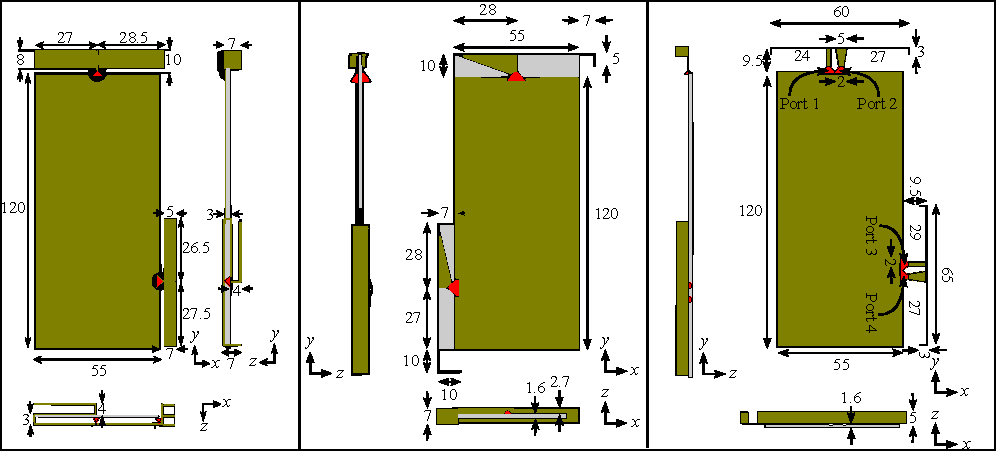
\includegraphics[width=\textwidth]{img/henrik/all_td}%

  \end{center}
\end{frame}

%\section{Free-space simulations}

\begin{frame}
    \frametitle{Free-space simulations -- Monopole (S-parameters)}
    \vspace*{-0.5cm}
  \begin{minipage}[t]{0.49\linewidth}
    \vspace{0mm}

    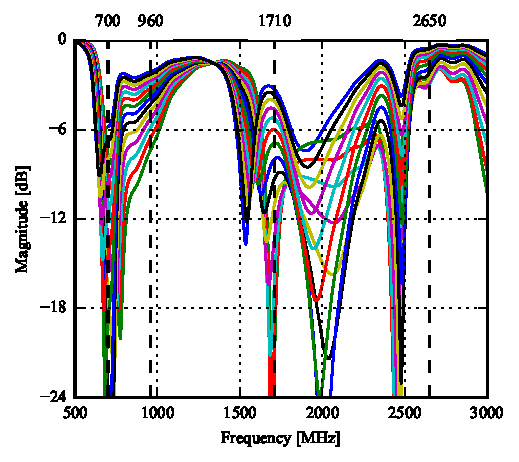
\includegraphics[width=0.78\linewidth]{img/henrik/mono/s11} \\
    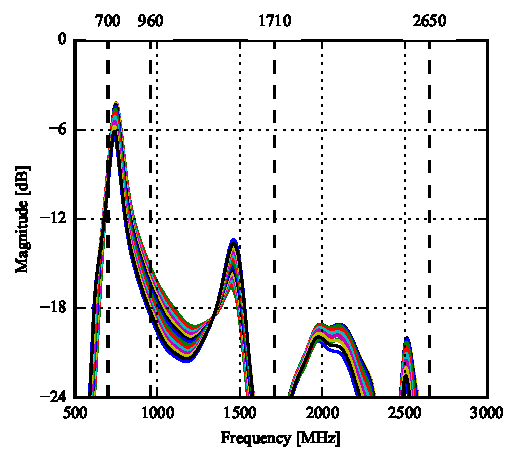
\includegraphics[width=0.78\linewidth]{img/henrik/mono/s21-s11} 

  \end{minipage}\hfill       
  \begin{minipage}[t]{0.49\linewidth}
    \vspace{0 mm}

    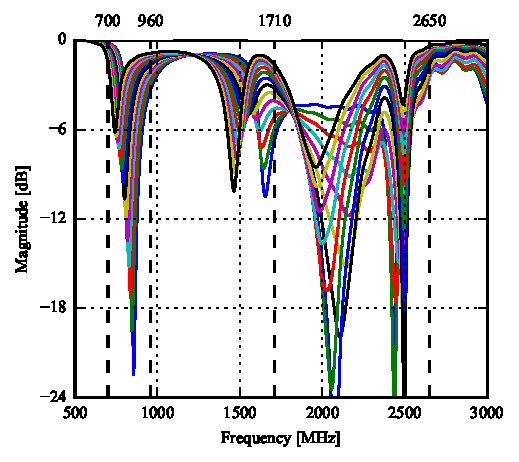
\includegraphics[width=0.78\linewidth]{img/henrik/mono/s22} \\
    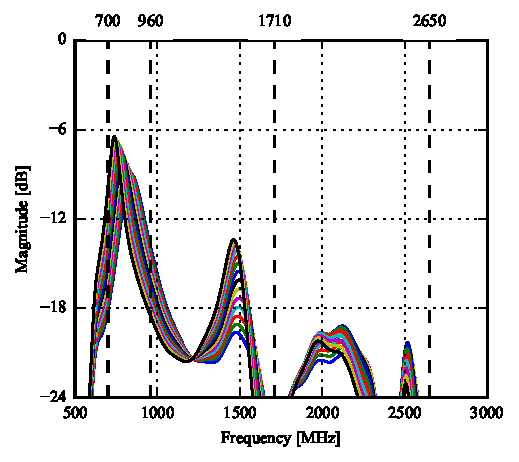
\includegraphics[width=0.78\linewidth]{img/henrik/mono/s21-s22} 

  \end{minipage}    
\end{frame}

\begin{frame}
    \frametitle{Free-space simulations -- Monopole (Efficiency and correlation)}
    \vspace*{-0.5cm}
  \begin{minipage}[t]{0.49\linewidth}
    \vspace{0mm}

    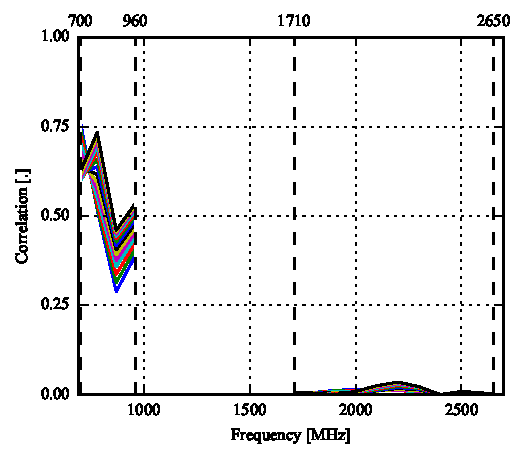
\includegraphics[width=0.78\linewidth]{img/henrik/mono/s11_corr} \\
    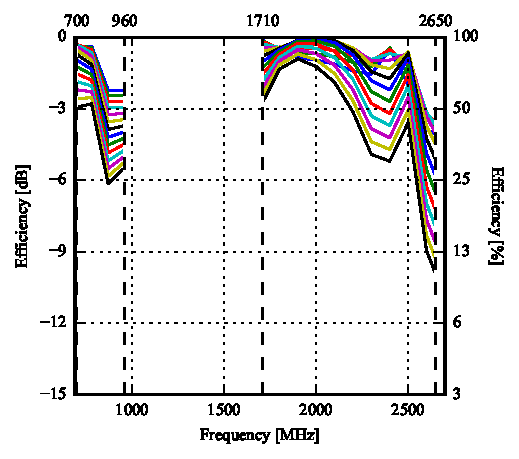
\includegraphics[width=0.82\linewidth]{img/henrik/mono/efficiency-ac1-csh1} 

  \end{minipage}\hfill       
  \begin{minipage}[t]{0.49\linewidth}
    \vspace{0 mm}

    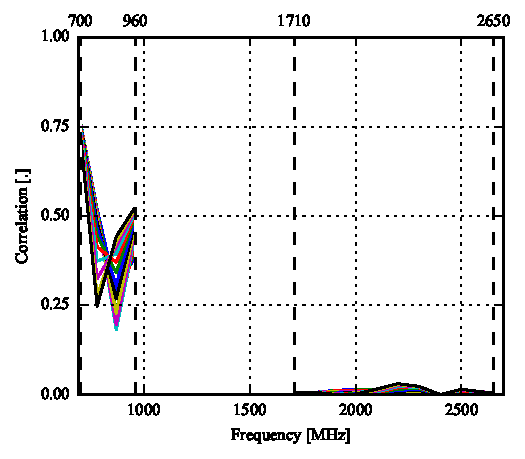
\includegraphics[width=0.78\linewidth]{img/henrik/mono/s22_corr} \\
    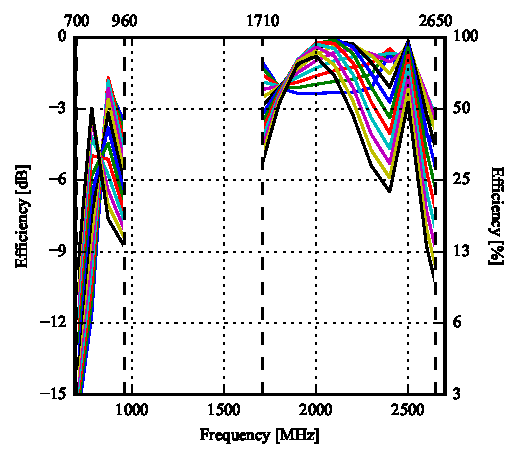
\includegraphics[width=0.82\linewidth]{img/henrik/mono/efficiency-ac2-csh2} 

  \end{minipage}    
\end{frame}



\begin{frame}
    \frametitle{Free-space simulations -- Triangle-feed (S-parameters)}
    \vspace*{-0.5cm}
  \begin{minipage}[t]{0.49\linewidth}
    \vspace{0mm}

    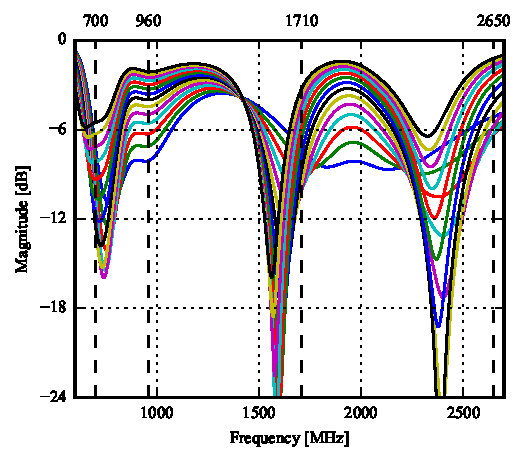
\includegraphics[width=0.78\linewidth]{img/henrik/triag/Csh1s11.pdf} \\
    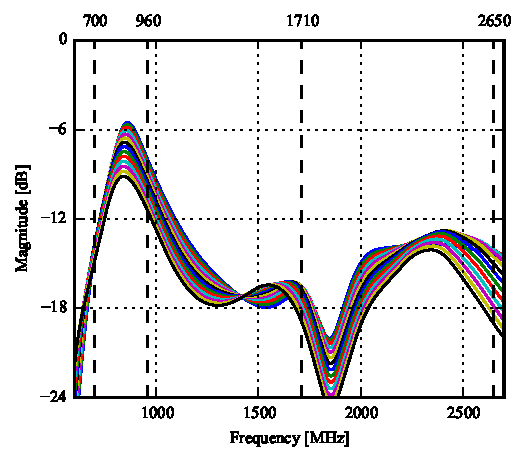
\includegraphics[width=0.78\linewidth]{img/henrik/triag/Csh1s21.pdf} 

  \end{minipage}\hfill       
  \begin{minipage}[t]{0.49\linewidth}
    \vspace{0 mm}

    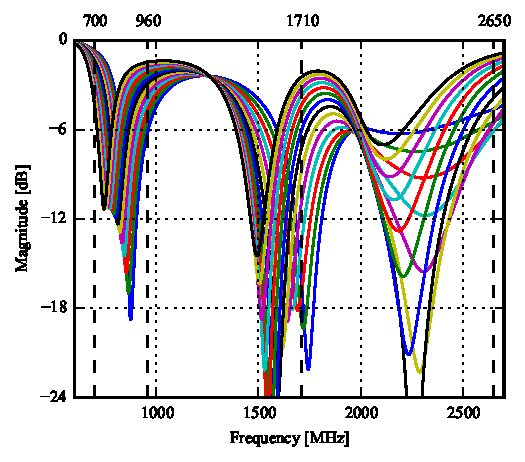
\includegraphics[width=0.78\linewidth]{img/henrik/triag/Csh2s22.pdf} \\
    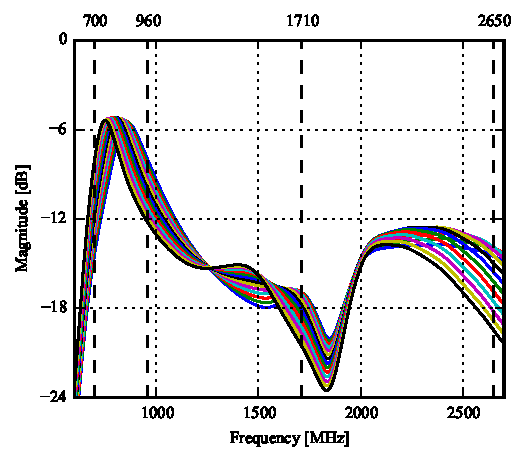
\includegraphics[width=0.78\linewidth]{img/henrik/triag/Csh2s21.pdf} 

  \end{minipage}    


\end{frame}

\begin{frame}
    \frametitle{Free-space simulations -- Triangle-feed (Efficiency and correlation)}
    \vspace*{-0.5cm}
  \begin{minipage}[t]{0.49\linewidth}
    \vspace{0mm}

    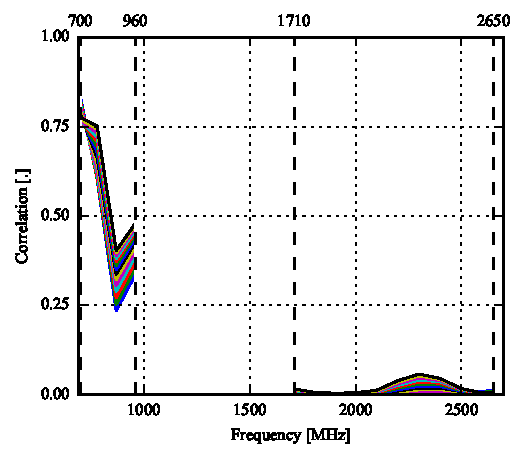
\includegraphics[width=0.78\linewidth]{img/henrik/triag/correlation_Csh1-sweep} \\
    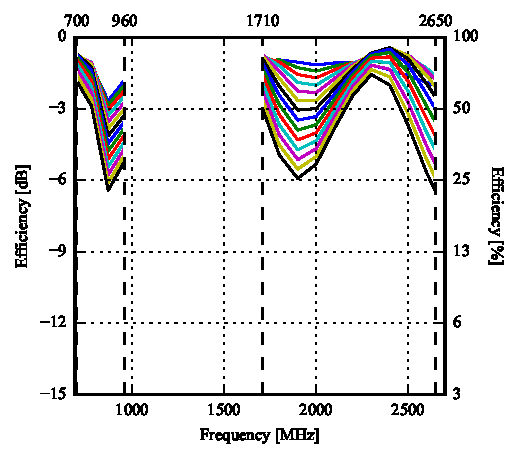
\includegraphics[width=0.78\linewidth]{img/henrik/triag/efficiency-ac1-csh1.pdf} \\



  \end{minipage}\hfill       
  \begin{minipage}[t]{0.49\linewidth}
    \vspace{0 mm}

    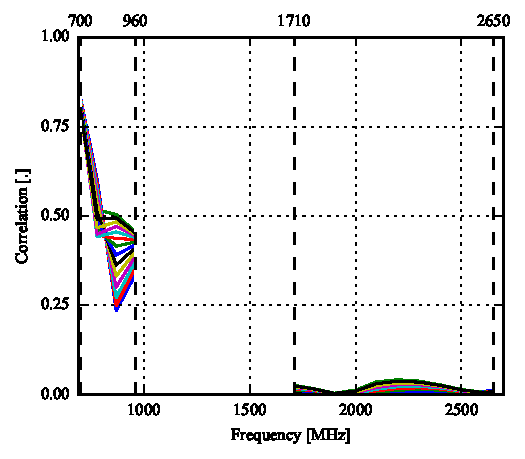
\includegraphics[width=0.78\linewidth]{img/henrik/triag/correlation_Csh2-sweep} \\
    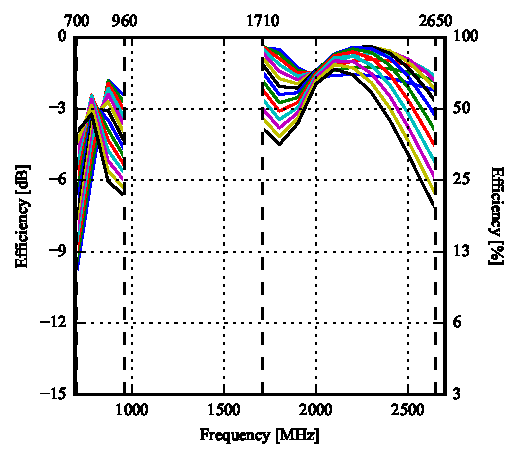
\includegraphics[width=0.78\linewidth]{img/henrik/triag/efficiency-ac2-csh2.pdf} 


  \end{minipage}    

\end{frame}


\begin{frame}
    \frametitle{Free-space simulations -- Dual-port (S-parameters)}

    \vspace*{-0.5cm}
  \begin{minipage}[t]{0.49\linewidth}
    \vspace{0mm}

    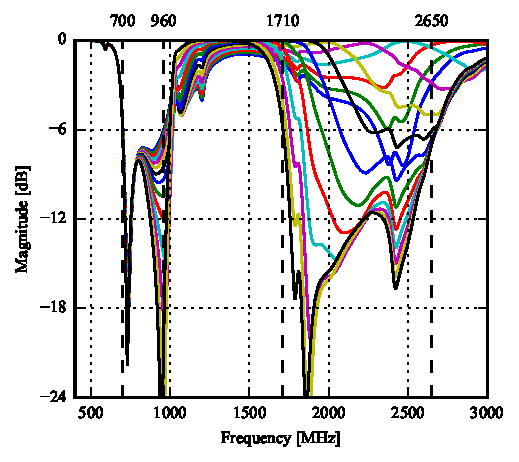
\includegraphics[width=0.78\linewidth]{img/henrik/dp/s11_top_sweep.pdf} \\
    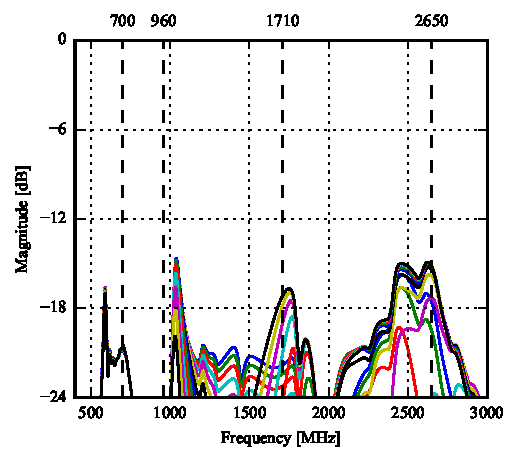
\includegraphics[width=0.78\linewidth]{img/henrik/dp/s12_top_sweep.pdf} 

  \end{minipage}\hfill       
  \begin{minipage}[t]{0.49\linewidth}
    \vspace{0 mm}

    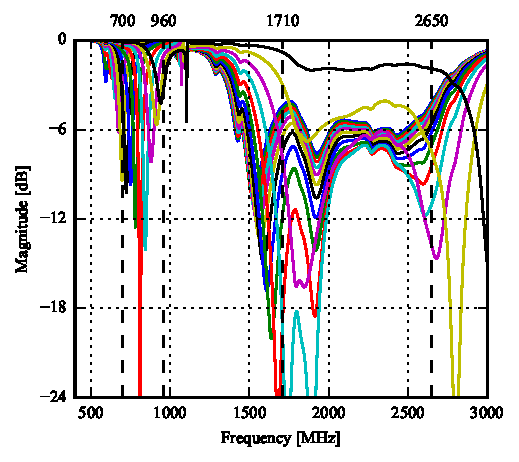
\includegraphics[width=0.78\linewidth]{img/henrik/dp/s22_side_sweep.pdf} \\
    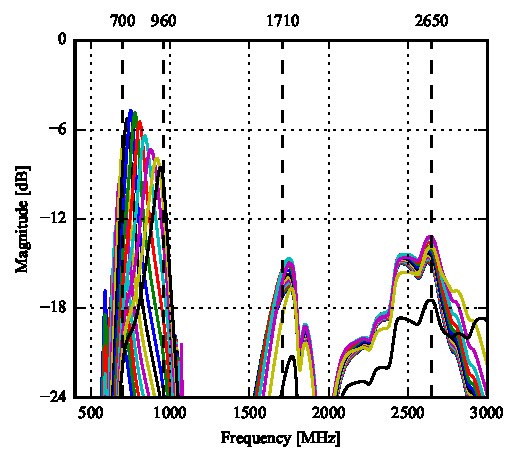
\includegraphics[width=0.78\linewidth]{img/henrik/dp/s21_side_sweep.pdf} 

  \end{minipage}    



\end{frame}

\begin{frame}
    \frametitle{Free-space simulations -- Dual-port (Efficiency and correlation)}
    \vspace*{-0.5cm}
  \begin{minipage}[t]{0.49\linewidth}
    \vspace{0mm}

    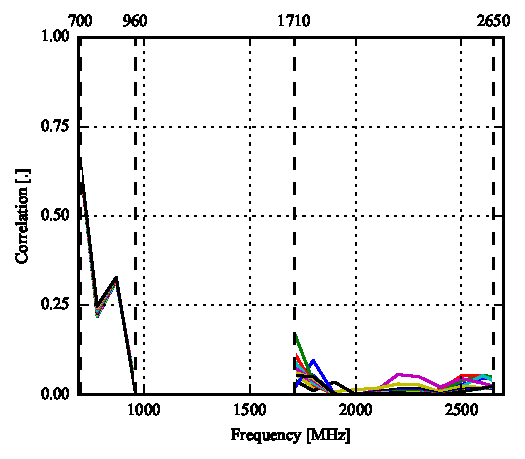
\includegraphics[width=0.78\linewidth]{img/henrik/dp/sweep_top_corr} \\
    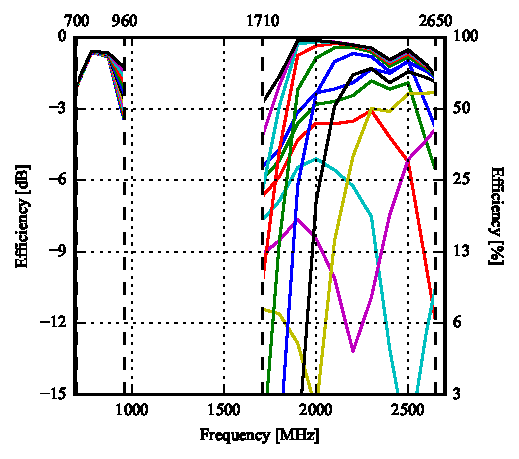
\includegraphics[width=0.78\linewidth]{img/henrik/dp/efficiency-ac2-top.pdf} 

  \end{minipage}\hfill       
  \begin{minipage}[t]{0.49\linewidth}
    \vspace{0 mm}

    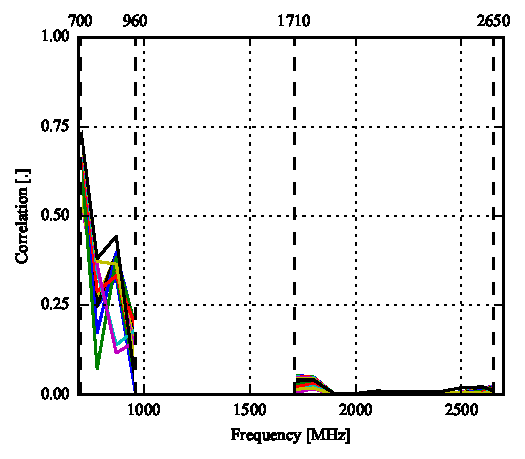
\includegraphics[width=0.78\linewidth]{img/henrik/dp/sweep_side_corr} \\
    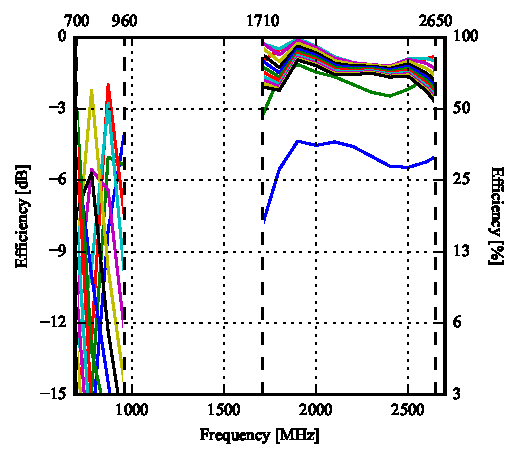
\includegraphics[width=0.78\linewidth]{img/henrik/dp/efficiency-ac3-side.pdf} 

  \end{minipage}    

\end{frame}









